\chapter{Создание макета системы управления микроклиматом теплицы}

\section{Условное графическое представление макета с разбиением на функциональные и структурные блоки}

Функционально макет можно разделить на ряд блоков, каждый из которых будет представлять собой подсистему. Функциональная схема данного макета представлена на рис.~\ref{fig:func_schem}.

\begin{figure}[H]
    \centering
    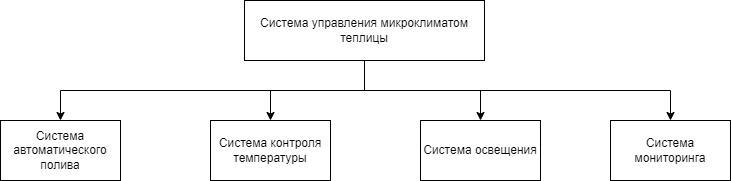
\includegraphics[scale=0.6]{images/system_schem.png}
    \caption{Функциональная схема макета умной теплицы.}
    \label{fig:func_schem}
\end{figure}

Структурная схема макета дает лучшее представление о последовательности взаимодействия функциональных частей макета и представлена на рис.~\ref{fig:struct_schem}.

\begin{figure}[H]
    \centering
    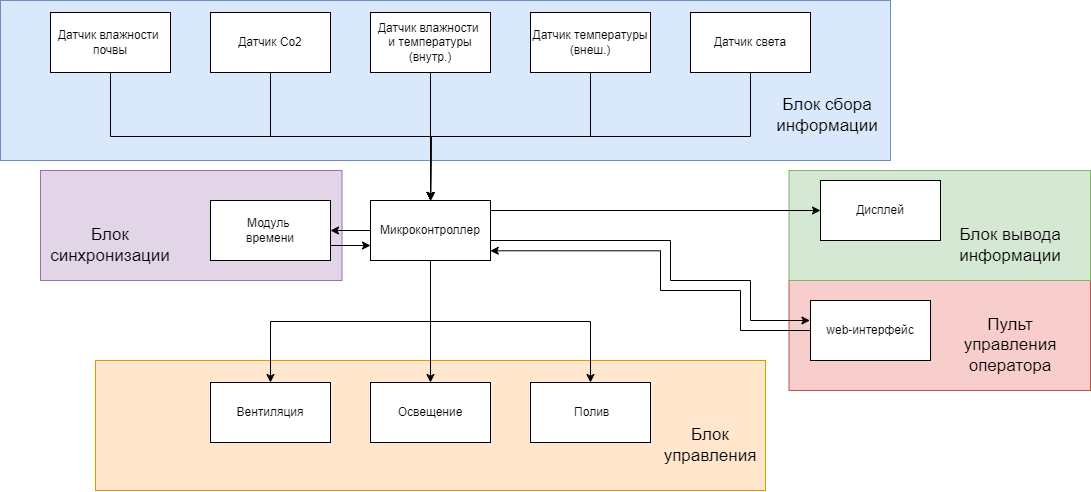
\includegraphics[scale=0.4]{images/struct_schem.png}
    \caption{Структурная схема макета умной теплицы.}
    \label{fig:struct_schem}
\end{figure}

\subsection{Модуль управления макетом}

Модуль управления макетом состоит из контроллера ESP32. Его краткие технические характеристики приведены в таблице:

\begin{table}[H]
    \centering
    \begin{tabular}{|p{6.5cm}|p{7.5cm}|}
        \hline
        Название & Характеристика \\
        \hline
        Микрокопроцессор & 32-битный Xtensa dual-core 2 ядра \\
        \hline
        Частота процессора & 160-240 МГц \\
        \hline
        ОЗУ & 520 КБ \\
        \hline
        ПЗУ & 448 КБ \\
        \hline
        Память программ & 4 МБ \\
        \hline
        RTC таймер & 16 КБ ОЗУ \\
        \hline
        Напряжение питания & 2,2-3,6 В \\
        \hline
        АЦП & 12 бит, 18 портов \\
        \hline
        ЦАП & 8 бит, 2 порта \\
        \hline
        Температурный датчик & есть \\
        \hline
        UART & есть, 3 шт. \\
        \hline
        SPI & естьб 4 шт. \\
        \hline
        IS1 & есть, 2 шт. \\
        \hline
        I2C & есть, 2 шт. \\
        \hline
        Максимальный ток при передача Wi-Fi & 160-260 мА \\
        \hline
        Потребление тока без Wi-Fi и Bluetooth & 20 мА \\
        \hline
        Wi-Fi & 802.11n 2.4 Гц, максимальная скорость 150 Мбит/сек \\
        \hline
        Bluetooth & v4.2 BR/EDR and BLE \\
        \hline
        Габариты & 26×18×5 мм \\
        \hline
        Вес & 8 г \\
        \hline
    \end{tabular}
    \label{tab:esp}
\end{table}

Управляющий контроллер ESP32 --- это микроконтроллер, разработанный компанией Espressif Systems. Он используется в широком спектре устройств, включая умные дома, умные гаджеты, Интернет вещей (IoT) и т.д. Одной из его главных особенностей является интеграция беспроводных технологий, таких как Wi-Fi и Bluetooth;

\begin{figure}[H]
    \centering
    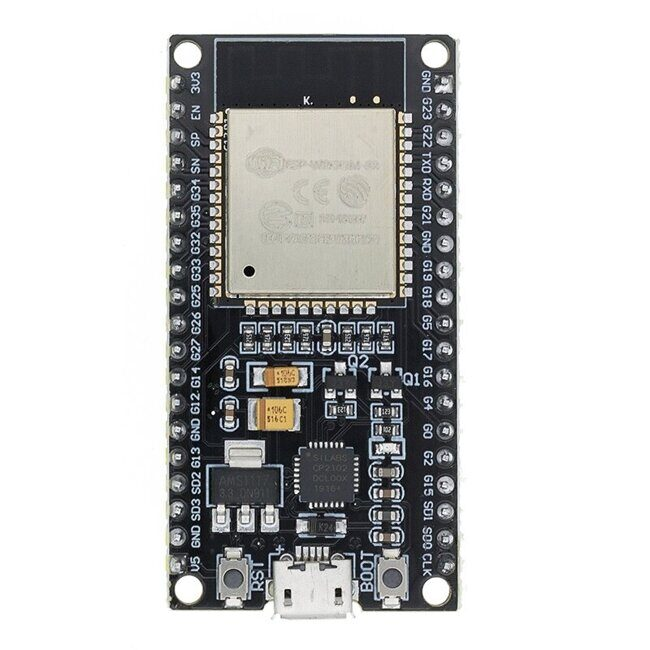
\includegraphics[scale=0.45]{images/esp.jpg}
    \caption{Управляющий контроллер ESP-32(отладочная плата).}
    \label{fig:esp}
\end{figure}

\subsection{Модуль измерения параметров окружающей среды}

Данная Модуль представляет из себя набор различных датчиков для измерения параметров окружающей среды, среди которых:

\begin{enumerate}
    \item емкостной датчик влажности почвы;

    \begin{figure}[H]
        \centering
        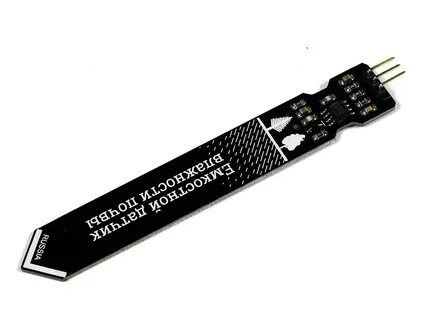
\includegraphics[scale=0.6]{images/wet.jpg}
        \caption{Емкостной датчик влажности почвы.}
        \label{fig:wet}
    \end{figure}
    
    Его краткие технические характеристики приведены ниже:

    \begin{table}[H]
        \centering
        \begin{tabular}{|p{6.5cm}|p{6.5cm}|}
            \hline
            Название & Характеристика \\
            \hline
            Тип датчика & ёмкостный \\
            \hline
            Напряжение питания & 3,3-5 В \\
            \hline
            Потребляемый ток & 6 мА \\
            \hline
            Интерфейс & аналоговый сигнал \\
            \hline
            Диапазон выходного сигнала & 0,5-3,3 В \\
            \hline
            Глубина погружения в почву & до 80 мм \\
            \hline
            Габариты & 118×20×7,6 мм \\
            \hline
        \end{tabular}
        \label{tab:wet}
    \end{table}

    \item датчик углекислого газа MQ-7;

    \begin{figure}[H]
        \centering
        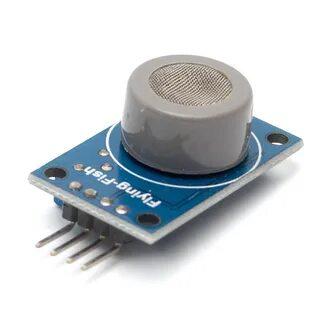
\includegraphics[scale=0.5]{images/mq7.jpg}
        \caption{Датчик Co2 MQ-7.}
        \label{fig:mq7}
    \end{figure}
    
    Его краткие технические характеристики приведены ниже:

    \begin{table}[H]
        \centering
        \begin{tabular}{|p{6.5cm}|p{6.5cm}|}
            \hline
            Название & Характеристика \\
            \hline
            Диапазон чувствительности & 10-10000 ppm \\
            \hline
            Напряжение питания & 5 В \\
            \hline
            Потребляемый ток & 160 мА \\
            \hline
            Напряжение нагревателя & 1,5-5 В \\
            \hline
            Время накала нагревателя & 60-90 сек \\
            \hline
            Сопротивление нагревателя & 31 Ом \\
            \hline
            Мощность нагревателя & 330 мВт \\
            \hline
            Сопротивление датчика & 2-20 кОм \\
            \hline
            Рабочая температура & от -10 до
            +50 \degree C \\
            \hline
            Рабочая влажность & <=95 \% \\
            \hline
            Концентрация кислорода & 21 \% \\
            \hline
            Габариты & 22×22×17 мм \\
            \hline
            Вес модуля & 5 г \\
            \hline
        \end{tabular}
        \label{tab:mq7}
    \end{table}
    
    \item датчик влажности воздуха и температуры DHT11;

    \begin{figure}[H]
        \centering
        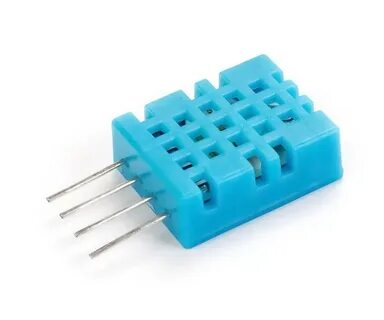
\includegraphics[scale=0.6]{images/dht11.jpg}
        \caption{Датчик влажности и температуры DHT11.}
        \label{fig:dht11}
    \end{figure}
    
    Его краткие технические характеристики приведены ниже:

    \begin{table}[H]
        \centering
        \begin{tabular}{|p{6.5cm}|p{6.5cm}|}
            \hline
            Название & Характеристика \\
            \hline
            Диапазон измерений влажности, погрешность & от 20 до 80\%, до 5\% \\
            \hline
            Диапазон измерения температур, погрешность & от 0 до 50 \degree C, 2\% \\
            \hline
            Напряжение питания & 3-5 В \\
            \hline
            Потребляемый ток & 2,5 мА \\
            \hline
            Частота работы & 1 Гц \\
            \hline
            Габариты & 15,5×12×5,5 мм \\
            \hline
        \end{tabular}
        \label{tab:dht11}
    \end{table}
    
    \item датчик освещенности BH1750;

    \begin{figure}[H]
        \centering
        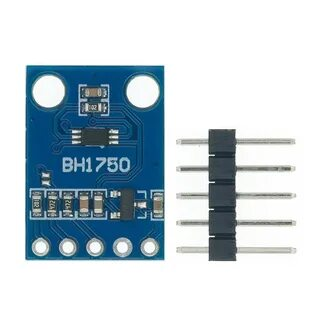
\includegraphics[scale=0.6]{images/bh1750.jpg}
        \caption{Датчик освещенности BH1750.}
        \label{fig:bh1750}
    \end{figure}
    
    Его краткие технические характеристики приведены ниже:

    \begin{longtable}{|p{6.5cm}|p{6.5cm}|}
        \hline
        Название & Характеристика \\
        \hline
        Интерфейс & I2C \\
        \hline
        Напряжение питания & 5 В \\
        \hline
        Чип & BH1750FVI \\
        \hline
        АЦП & 16 бит \\
        \hline
        Точность & 1 люкс \\
        \hline
        Чувствительность & 65536 градаций \\
        \hline
        Калибровка & не требуется \\
        \hline
        Габариты & 118×20×7,6 мм \\
        \hline
        Вес & 5 г \\
        \hline
    \end{longtable}
    \label{tab:bh1750}
    
    \item датчик температуры (внешний) DS18B20;

    \begin{figure}[H]
        \centering
        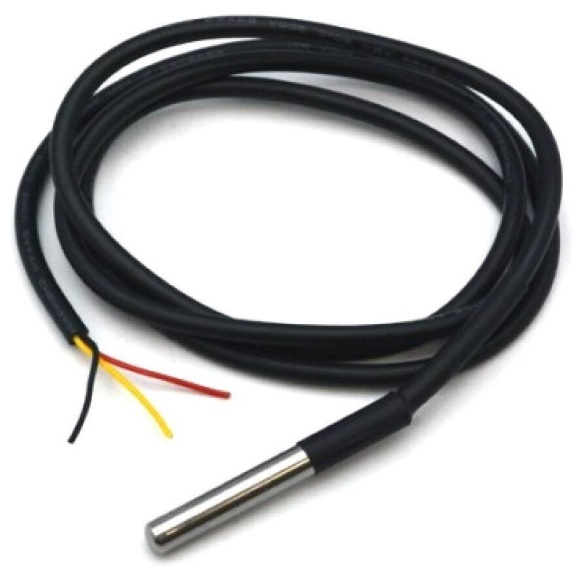
\includegraphics[scale=0.8]{images/temperature.jpg}
        \caption{Датчик температуры DS18B20.}
        \label{fig:temp}
    \end{figure}
    
    Его краткие технические характеристики приведены ниже:

    \begin{table}[H]
        \centering
        \begin{tabular}{|p{7cm}|p{6.5cm}|}
            \hline
            Название & Характеристика \\
            \hline
            Диапазон измерения температур & от -55 до +125 \degree C \\
            \hline
            Напряжение питания & 3,3-5 В \\
            \hline
            Количество датчиков на одной линии связи & до 127 \\
            \hline
            Протокол передачи & 1-Ware \\
            \hline
            Калибровка & не требуется \\
            \hline
        \end{tabular}
        \label{tab:temp}
    \end{table}
\end{enumerate}

\subsection{Модуль отображения параметров среды}

В качестве подсистемы отображения параметров окружающей среды выступает LCD-дисплей и модуль часов реального времени для точной привязки показаний к текущему времени.

LCD-дисплей 1602 --- это тип жидкокристаллического дисплея, который имеет 2 строки и 16 символов в каждой строке;

\begin{figure}[H]
    \centering
    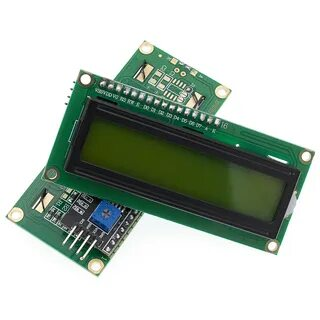
\includegraphics{images/lcd.jpg}
    \caption{LCD дисплей 1602.}
    \label{fig:lcd}
\end{figure}

Его краткие технические характеристики приведены ниже:

\begin{table}[H]
    \centering
    \begin{tabular}{|p{6.5cm}|p{6.5cm}|}
        \hline
        Название & Характеристика \\
        \hline
        Тип отображения & символьный \\
        \hline
        Загрузка новых символов & есть \\
        \hline
        Подсветка & есть \\
        \hline
        Контроллер & HD44780; \\
        \hline
        Напряжение питания & 5 В \\
        \hline
        Формат & 16 символов, 2 строки \\
        \hline
        Диапазон рабочих температур & от -20 до +70 \degree C \\
        \hline
        Угол обзора & 180 \degree \\
        \hline
    \end{tabular}
    \label{tab:lcd}
\end{table}

Модуль часов реального времени DS1307 --- это устройство, которое можно подключить к плате, чтобы обеспечить точное хранение и отслеживание времени;

\begin{figure}[H]
    \centering
    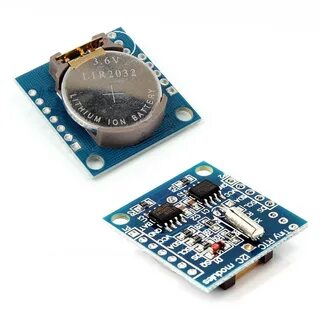
\includegraphics[scale=0.6]{images/ds1307.jpg}
    \caption{Модуль часов реального времени.}
    \label{fig:ds1307}
\end{figure}

Его краткие технические характеристики приведены ниже:

\begin{table}[H]
    \centering
    \begin{tabular}{|p{6.5cm}|p{6.5cm}|}
        \hline
        Название & Характеристика \\
        \hline
        Диапазон рабочих температур & от -40 до +85 \degree C \\
        \hline
        Напряжение питания & 5 В \\
        \hline
        Объём памяти & 56 байт \\
        \hline
        Режимы работы & 12-ти и 24-х часовой \\
        \hline
        Интерфейс & I2C \\
        \hline
    \end{tabular}
    \label{tab:ds1307}
\end{table}

\subsection{Модуль элементов поддержания параметров теплицы}

Для поддержания необходимых параметров окружающей среды в макете используются:

\begin{enumerate}
    \item вентиляция (куллеры);
    
    \item система полива (помпа) AD20P-1230C. Помпа AD20P-1230C – это компактная насосная станция, которая используется для перекачки воды и других жидкостей. Она может применяться в различных областях, включая бытовую и промышленную сферы. Помпа имеет компактные размеры и небольшой вес, что облегчает установку и транспортировку, низкий уровень шума работы, высокую производительность и эффективность;

    \begin{figure}[H]
        \centering
        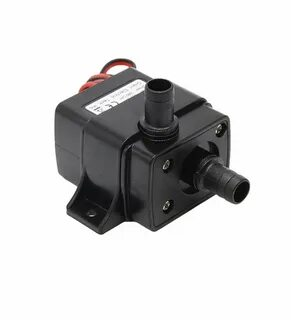
\includegraphics[scale=0.6]{images/pump.jpg}
        \caption{Помпа AD20P-1230C.}
        \label{fig:pump}
    \end{figure}
    
    \item система освещения (Светодиодная лента) IP65. Фитолента IP65 –-- это специальная светодиодная лента, разработанная для обеспечения растений в теплицах, оранжереях и других закрытых помещениях необходимым количеством света для нормального роста и развития.

    \begin{figure}[H]
        \centering
        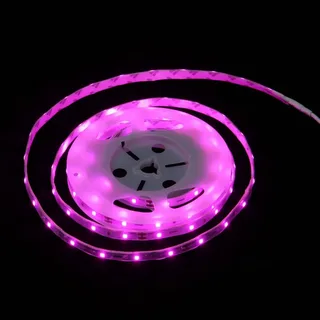
\includegraphics[scale=0.8]{images/ip65.png}
        \caption{Фитолента IP65.}
        \label{fig:ip65}
    \end{figure}
    
    Фитолента IP65 обладают следующими характеристиками:
    
    \begin{enumerate}
        \item устойчивость к влаге и пыли благодаря защитному покрытию IP65;
        \item высокая яркость светодиодов для обеспечения необходимого уровня освещения растений;
        \item низкое потребление электроэнергии;
        \item возможность регулировки яркости и цветовой температуры;
        \item гибкость и легкость монтажа на любой поверхности;
        \item долгий срок службы и надежность работы.
    \end{enumerate}
\end{enumerate}

Схема соединений для данного макета иллюстрирует связи входных и выходных элементов и устройств и представлена на рис.~\ref{fig:connection_schem} в Приложении А.

\section{Основные технические требования к макету}

Список требований, которые предъявляются к макету:
\begin{enumerate}
    \item назначение программной части макета: регулирование микроклимата в теплице;
    \item оборудование --- персональный компьютер следующими минимальными характеристиками:
    \begin{enumerate}
        \item ОЗУ: не менее 4 Гб;
        \item версия ОС: Windows 10 или новее, Linux 6.0 или новее;
        \item монитор с разрешением не менее 1280х1024;
        \item устройство ввода;
        \item устройство вывода звука;
        \item звуковая карта.
    \end{enumerate}
\end{enumerate}

\section{Описание работы макета}

Работу макета системы управления микроклиматом теплицы можно разбить на последовательность шагов и представить следующим образом:

\begin{enumerate}
    \item система подключается к источнику сети Wi-Fi;
    \item система получает собственный IP адрес в этой сети;
    \item система получает показания с датчиков и обрабатывает их;
    \item обработанные данные отображаются на LCD дисплее, а также в Web-интерфейсе;
    \item автоматическое регулирование происходит исходя из поставленных задач, заданных пользователем с помощью Web-интерфейса;
    \item ручное регулирование происходит с помощью ползунков отображаемых в Web-интерфейсе. 
\end{enumerate}

\section{Описание требований к функционалу макета}

К разработанному макету применяется ряд требований к функциональным возможностям:

\begin{enumerate}
    \item классификация уровня влажности почвы (очень сухая, сухая, сбалансированная, влажная, очень влажная);
    \item измерение относительной влажности воздуха (в процентах);
    \item измерение температуры воздуха в диапазоне от 0 до 40 градусов Цельсия;
    \item измерение освещенности в диапазоне от 0 до 20000 люкс;
    \item определение избыточного содержания $CO_2$ в воздухе;
    \item измерение температуры воздуха за пределами теплицы в диапазоне от -30 до 50 градусов Цельсия;
    \item наличие графического Web-интерфейса для отображения получаемых показателей, а также регулирования системы.
\end{enumerate}

\section{Тестирование макета}

% TODO: Разработать план тестирования работоспособности всех компонентов макета (будет обговариваться позже)